\documentclass[11pt]{article}
\usepackage{geometry}
\usepackage{graphicx}
\usepackage{enumitem}
\usepackage{float}
\usepackage{amsmath}
\usepackage{multicol}
\usepackage{cancel}

\geometry{a4paper, top=0.5in, bottom=0.5in, right=0.75in, left=0.75in}

\title{Lecture 3}
\author{}
\date{}

\begin{document}

\maketitle

\section{Introduction}
We have to study Einstein model since the classical model has the following limitations:
\begin{itemize}
    \item It considers light as a plane wave (not photons).
    \item It considers the energy of the atoms to be continuous and frequency-independent.
    \item Materials can only cause attenuation of incident light.
\end{itemize}
In modern physics, there are discrete energy levels, and the number of atoms in each level follows the Boltzmann distribution. Also, the energy is frequency-dependent ($E = h\nu$).
\begin{center}
    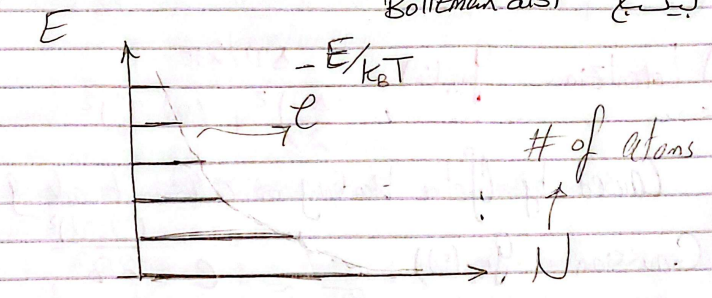
\includegraphics[scale=0.7]{1.png}
\end{center}


\section{Einstein Model}
Einstein model is based on the following assumptions:
\begin{itemize}
    \item There are only 2 levels ($E_1$ and $E_2$) with number of atoms $N_1$ and $N_2$ respectively. 
    \item Incident light will only interact at the resonance frequency ($\nu_0$), where $E_2 - E_1 = h\nu_0$.
\end{itemize} 

\subsection{Light-Matter Interaction}
\subsubsection{Absorption}
\begin{itemize}
    \item The atom absorbs a photon and moves from $E_1$ to $E_2$.
    \item The rate of absorption is given by:
    \begin{equation*}
        \frac{dN_2}{dt} \bigg|_{\text{abs}} = B_{12} \rho N_1   
    \end{equation*}
    where:
    \begin{itemize}
        \item $B_{12}$ is the Einstein coefficient for absorption.
        \item $\rho$ is the energy density per unit frequency
    \end{itemize}
\end{itemize}
\begin{center}
    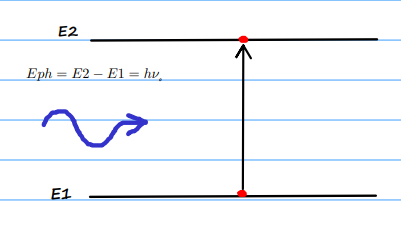
\includegraphics[scale=0.8]{2.png}
\end{center}

\subsubsection{Spontaneous Emission}
\begin{itemize}
    \item The atom moves from $E_2$ to $E_1$ and emits a photon of different phase and frequency from the incident photon (noise photons).
    \item The rate of spontaneous emission is given by:
    \begin{align*}
        \frac{dN_2}{dt} \bigg|_{\text{spon}} &= -A_{21} N_2 \\
        N_2(t) &= N_2(0) e^{-A_{21}t}
    \end{align*}
\end{itemize}
\begin{center}
    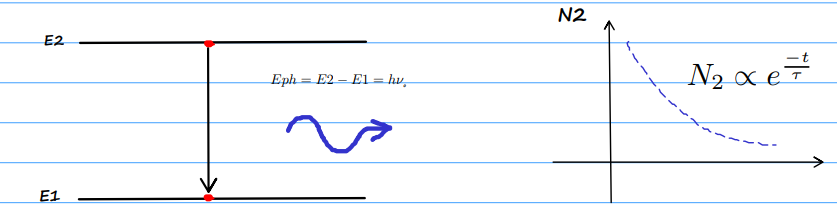
\includegraphics[scale=0.8]{3.png}
\end{center}


\subsubsection{Stimulated Emission}
\begin{itemize}
    \item An incident photon will not be absorbed \& move normally through the material, but it triggers the atom to move from $E_2$ to $E_1$ and emit a photon of the same frequency, phase and polarization. 
    \item This can be explained by Maxwell's equations' time reversability. This property states that there is a solution to Maxwell's equations for time (t = -t). So, stimulated emission is the time-reversed version for this scenario: There are 2 incident photons, and one is absorbed by the atom, so the other one will pass through the material.
    \item The rate of stimulated emission is given by:
    \begin{align*}
        \frac{dN_2}{dt} \bigg|_{\text{stim}} = -B_{21} \rho N_2
    \end{align*}
\end{itemize}
\begin{center}
    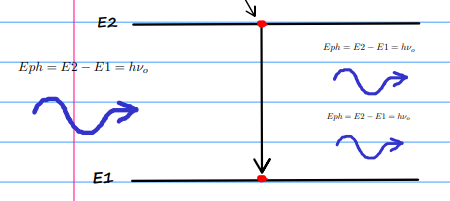
\includegraphics[scale=1]{4.png}
\end{center}

\subsection{Steady State Analysis}
\begin{itemize}
    \item We want to find a compact form for energy density $\rho$ at steady state thermal equilibrium.
    \item  Note that this doesn't necessarily mean that it is static equilibrium (no atoms are moving), but it means that the system is in a state where the number of atoms in each level is constant (total number of atoms moving down is equal to the total number of atoms moving up).
    \item At steady state, there is no change in energy, so input energy (excitation) = output energy (radiation). 
    \item Note that the following equations only represent the rate of change in $N_2$ from radiation only (no collision or other sources).
\end{itemize}
\begin{align*}
    \frac{dN_2}{dt} = \frac{dN_2}{dt} \bigg|_{\text{abs}} + \frac{dN_2}{dt} \bigg|_{\text{spon}} + \frac{dN_2}{dt} \bigg|_{\text{stim}} = 0 \\
    -A_{12} N_2 + B_{21} \rho N_2 + B_{12} \rho N_1 = 0 
\end{align*}
So:
\begin{align*}
    B_{12} \rho N_1 &= N_2 (B_{21} \rho + A_{21}) \\
    \frac{N_2}{N_1} &= \frac{B_{12} \rho}{A_{21} + B_{21} \rho}
\end{align*}
$\frac{N_2}{N_1}$ follows the Boltzmann distribution, so:
\begin{align*}
    e^{-\frac{h\nu}{k_BT}} &= \frac{B_{12} \rho}{A_{21} + B_{21} \rho} \\
\end{align*}
Divide by $\frac{B_{12} \rho}{B_{12} \rho}$:
\begin{align*}
    e^{-\frac{h\nu}{k_BT}} &= \frac{1}{\frac{A_{21}}{B_{12} \rho} + \frac{B_{21}}{B_{12}}} \\
    \frac{A_{21}}{B_{12} \rho} &= e^{\frac{h\nu}{k_BT}} - \frac{B_{21}}{B_{12}} \\
\end{align*}
Multiply by $\frac{B_{12}}{B_{21}}$:
\begin{align*}
    \frac{A_{21}}{B_{21}} \frac{1}{\rho} &= \frac{B_{12}}{B_{21}} e^{\frac{h\nu}{k_BT}} - 1 
\end{align*}
So:
\begin{align*}
    \rho &= \frac{A_{21}}{B_{21}} \frac{1}{\frac{B_{12}}{B_{21}} e^{\frac{h\nu}{k_BT}} - 1} 
\end{align*}
Compare with Planck's black body radiation equation:
\begin{align*}
    \rho &= \frac{8\pi n^3 h\nu^3}{c_0^3} \frac{1}{e^{\frac{h\nu}{k_BT}} - 1} \\
    &\implies B_{12} = B_{21} = B \\
    &\implies \frac{A}{B} = \frac{8\pi n^3 h\nu^3}{c_0^3}
\end{align*}
Using $c = \frac{c_0}{n}$ and $c = \lambda \nu$:
\begin{align*}
    \frac{A}{B} = \frac{8 \pi h}{\lambda^3}
\end{align*}
$A$ represents the spontaneous emission, so:
\begin{align*}
    A &= \frac{1}{\tau_r} \\
    B &= \frac{\lambda^3}{8\pi h \tau_r}
\end{align*}
Remarks:
\begin{itemize}
    \item It is reasonable for $B_{12} = B_{21}$ since the probability of absorption and stimulated emission should be the same.
    \item Similar to $A_{21} = \frac{1}{\tau_r}$, we can say that $B_{21} \rho = \frac{1}{\tau_{stim}}$ and $B_{12} \rho = \frac{1}{\tau_{abs}}$.
    \item Note that spontaneous emission is independent of the incident light, but stimulated emission and absorption is dependent on the incident light.
    \item Despite having the same probability, the rate of stimulated emission or absorption might differ depending on the number of atoms in each level.
\end{itemize}

\subsection{Energy Density \& Light Intensity}
Energy inside a volume per unit frequency (E) of an area (A):
\begin{align*}
    \text{E} &= \rho A \Delta z \\
\end{align*}
The time that energy takes to pass through the volume (T):
\begin{align*}
    \text{T} &= \frac{\Delta z}{v_g}
\end{align*}
Power per unit frequency (P):
\begin{align*}
    P &= \frac{E}{\text{T}} = \rho A  v_g
\end{align*}
Intensity per unit frequency (I):
\begin{align*}
    I &= \frac{P}{A} = \rho v_g
\end{align*}
Substitute $\rho = \frac{I}{v_g}$ in rate equations:
\begin{align*}
    \frac{dN_2}{dt} \bigg|_{\text{abs}} &= B \rho N_1 = B \frac{I}{v_g} N_1 \\
    \frac{dN_2}{dt} \bigg|_{\text{stim}} &= -B \rho N_2 = -B \frac{I}{v_g} N_2
\end{align*}
Intensity in terms of number of atoms:
\begin{align*}
    I &= \frac{P}{A} = \frac{\text{\# photons * photon energy}}{\text{area * time}} \\
    &= \frac{\text{\# photons}}{\text{area * time}} * h \nu = \phi h \nu\\
\end{align*}
where $\phi$ is the number of photons per unit area per unit time per unit frequency and named the photon flux density per unit frequency. \\
So:
\begin{align*}
    \text{absorption rate} &= \frac{1}{\tau_{abs}} = B \frac{I}{v_g} = B \frac{\phi h \nu}{v_g} \\
    \text{stimulated rate} &= \frac{1}{\tau_{stim}} = -B \frac{I}{v_g} = -B \frac{\phi h \nu}{v_g}
\end{align*}
Given that $v_g = \frac{1}{\partial \beta / \partial \omega}$ and $\beta = n(\omega) \frac{\omega}{c_0}$:
\begin{align*}
    \frac{1}{v_g} &= \frac{n}{c_0} + \frac{\omega}{c_0} \frac{\partial n}{\partial \omega} \\
    v_g &= c_0 \frac{1}{n + \omega \frac{\partial n}{\partial \omega}}
\end{align*}
Neglecting material dispersion ($\frac{\partial n}{\partial \omega} = 0$):
\begin{align*}
    v_g &= \frac{c_0}{n} = c
\end{align*}
So:
\begin{align*}
    \frac{B h \nu \phi}{v_g} &= \frac{B h \nu \phi}{c} = \frac{\lambda^3 \phi}{8 \pi h \tau_r} \frac{h \nu}{c} = \frac{\lambda^2 \phi}{8 \pi \tau_r}
\end{align*}

\section{Corrections to Einstein Model}
Einstein model does not acount for Heisenberg's uncertainty principle, which states that we cannot know the exact energy at a specific time ($\Delta E \Delta t \geq \frac{\hbar}{2}$). This means that there is no exact energy level ($E_2 + \Delta E$) for the electron to transition to, so each electron can gain different energy ($E=h \nu$) and still transition. So, we have to consider the line shape function $g_{\nu_0}(\nu)$. The corrected rate is given by:
\begin{align*}
    \text{rate} = \frac{\lambda^2 \phi}{8 \pi \tau_r} g_{\nu_0}(\nu) d\nu
\end{align*}
Let $\sigma = \frac{\lambda^2}{8 \pi \tau_r} g_{\nu_0}(\nu)$:
\begin{align*}
    \text{rate} = \sigma \phi_{\nu} 
\end{align*}
where $\phi_{\nu}$ is the photon flux density (not per unit frequency).
\subsection{Effect on Atomic Rates}
Recall that the line shape function is normalized (per unit frequency), so to get the total rate of change in number of atoms, we have to integrate over all frequencies.
\subsubsection{Spontaneous Emission}
Since it only depends on the lifetime in an energy level, it is independent of the incident light, so there is no effect:
\begin{align*}
    \frac{dN_2}{dt} \bigg|_{\text{spon}} = \int_{-\infty}^{\infty} -A_{21} N_2 g_{\nu_0}(\nu) d\nu = -A_{21} N_2
\end{align*}
\subsubsection{Stimulated Emission}
\begin{align*}
    \frac{dN_2}{dt} \bigg|_{\text{stim}} = \int_{-\infty}^{\infty} -B_{21} \rho N_2 g_{\nu_0}(\nu) d\nu
\end{align*}
We cannot exclude the $\rho$ term since it depends on the frequency-dependent incident light, so let's consider these 2 cases:
\begin{itemize}
    \item \textbf{White Source} 
        \begin{itemize}
            \item $\rho(\nu)$ FWHM $>> g_{\nu_0}(\nu)$ FWHM
            \item We can consider the line shape function as an impulse function ($\int_{-\infty}^{\infty} \rho(\nu) g_{\nu_0}(\nu) d\nu \approx \rho(\nu_0)$)
            \begin{align*}
                \frac{dN_2}{dt} \bigg|_{\text{stim}} &= -B_{21} N_2 \rho(\nu_0)
            \end{align*}
            \item In this case, Einstein model is valid.
        \end{itemize}
        \begin{center}
            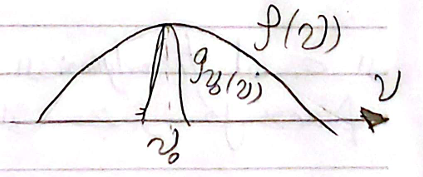
\includegraphics[scale=0.8]{5.png}
        \end{center}

    \item \textbf{Narrow Light Source}
        \begin{itemize}
            \item We cannot consider the source as an impulse since it is not normalized ($\int_{-\infty}^{\infty} \rho(\nu) d\nu \not= 1$), but we can consider it as a weighted impulse with a weight of $\rho_s$
            \begin{align*}
                \frac{dN_2}{dt} \bigg|_{\text{stim}} &= \int_{-\infty}^{\infty} -B_{21} N_2 \rho_s \delta(\nu - \nu_s) g_{\nu_0}(\nu) d\nu = -B_{21} N_2 \rho_s g_{\nu_0}(\nu_s)
            \end{align*}
            \item From the previous derivation:
            \begin{align*}
                \frac{dN_2}{dt} \bigg|_{\text{stim}} &= \sigma \phi_{\nu} N_2
            \end{align*}
        \end{itemize}
        \begin{center}
            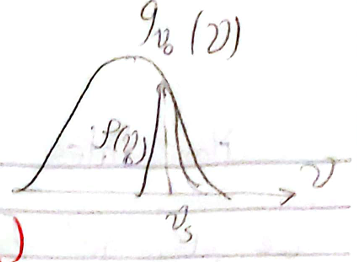
\includegraphics[scale=0.8]{6.png}
        \end{center}
\end{itemize}

\section{Conclusion}
\begin{itemize}
    \item We have an incident number of photons per unit area per unit time ($\phi_{\nu}(z)$) on a material, where absorption, spontaneous emission and stimulated emission can occur.
    \item We neglect the effect of spontaneous emission since it is random.
    \item We are intersted in the change in the number of photons after passing through the material, so:
\end{itemize}
\begin{align*}
    [\phi_{\nu}(z + \Delta z) - \phi_{\nu}(z)] * \text{Area} = [R_{stim}N_2 - R_{abs}N_1] * \text{Area} * \Delta z
\end{align*}
So:
\begin{align*}
    \frac{d\phi_{\nu}}{dz} &= R_{stim}N_2 - R_{abs}N_1 \\
    &= \sigma \phi_{\nu} N_2 - \sigma \phi_{\nu} N_1 \\
    &= \sigma \phi_{\nu} (N_2 - N_1) = \gamma \phi_{\nu} \\
\end{align*}
where $\gamma = \sigma (N_2 - N_1)$, so:
\begin{align*}
    \phi_{\nu}(z) = \phi_{\nu}(0) e^{\gamma z}
\end{align*}
\begin{itemize}
    \item Due to discretization of number of atoms in each level ($N_1$ and $N_2$ instead of $N_a$), amplification can occur if $N_2 > N_1$.
    \item At thermal equilibrium, $N_2 < N_1$.
\end{itemize}

\end{document}